
\documentclass[11pt, a4paper]{article}
\usepackage{german}

\usepackage{graphicx}
\usepackage{subcaption}

\usepackage[utf8]{inputenc}
\usepackage[T1]{fontenc}

\usepackage{tikz}
\usetikzlibrary{shapes.geometric, arrows}

\tikzstyle{io} = [trapezium, 
trapezium stretches=true,
trapezium left angle=70, 
trapezium right angle=110, 
minimum width=3cm, 
minimum height=1cm, text centered, 
draw=black, fill=blue!10]
\tikzstyle{process} = [rectangle, 
rounded corners,
minimum width=3cm, 
minimum height=1cm, 
text centered, 
text width=3cm, 
draw=black, 
fill=green!10]
\tikzstyle{arrow} = [thick,->,>=stealth]

\usepackage[
colorlinks=true, 
linkcolor=blue]{hyperref}

\usepackage{geometry}
\geometry{
    left=2.5cm,
    right=2.5cm,
    top=2.5cm,
    bottom=2.5cm}

\begin{document}
\author{Florian Röder, Yorick Behme, Dieter Nachname :)}
\title{KPMI Projektdokumentation}
\maketitle
\setcounter{tocdepth}{4}
\setcounter{secnumdepth}{4}
\tableofcontents

\newpage

\section{Einleitung}

\subsection{Projekthintergrund}

Das Projekt fand im Rahmen des Moduls INF-B-490 Komplexpraktikum Medieninformatik-Projekt im Zeitraum des Sommersemesters 2023 und Wintersemesters 2023/24 statt. 
Dabei diente das Sommersemester zum Einarbeiten in die jeweiligen Technologien via 'hands-on-Seminaren' in welchen jeweils ein Schwerpunkt beleuchtet wurde. 
Das Wintersemester 2023/24 diente der prototypischen Realisierung der Projektziele.\\
\\
Zielstellungen der Lehrveranstaltung beinhalten das praktische Kennenlernen von Mixed-Reality-Technologien und Physical Computing Ansätzen via Konzeption und Realisierung von Komponenten sowie Funktionen einer kombinierten Anwendung innerhalb eines 2–3-köpfigen Teams.\\
Genauer beschrieben ist das Ziel ein physisches Mensch-Computer-Interface, welches am Körper getragen werden kann, engl.: ''Wearable'' unter der Verwendung von e-Textile Sensoren prototypisch umzusetzen und dieses in eine Mixed-Reality beziehungsweise Augmented-Reality Applikation einzubinden.

\subsection{Projektüberblick}

Unser Projekt drehte sich um die Realisierung eines 'smartwatch-bracelet' Prototyps. 
Zentrale Ziele waren dabei die Erweiterung sowie Kombination der Eingabemodalitäten herkömmlicher 'Smartwatches'. 
Die Idee: Uhrenarmbänder, welche für gewöhnlich nur den Zweck verfolgen, die Uhr am Armgelenk zu befestigen, in die Interaktion mit der Smartwatch einzubinden und somit neue Interaktionsschnittstellen zu erforschen. 
Der Armband-Prototyp hat die Zielstellung auch ohne die Mixed-Reality Komponente eine Grundlage für eine erweiterte Smartwatch-Eingabeschnittstelle zu bilden.\\
Das Projekt lässt sich in 3 Teile unterteilen: Armband, Uhr, Augmented-Reality.


\subsection{Arbeitsteilung / Projektmanagement}

@TODO hier reinschreiben was íhr gemacht habt \\

Die 3 Bereiche wurden daraufhin auf die Gruppenmitglieder aufgeteilt. 
Yorick beschäftigte sich mit der Smartwatch App , sowie Teilen der Augmented Reality Visualisierung. 
Dieter ist für die Augmented Reality Visualisierung zuständig und Florian beschäftigte sich mit dem Entwurf und Design des Uhrenarmbands, die Verarbeitung der Sensordaten auf Arduino Seite sowie dessen Gegenpart auf der Unity Seite, sowie der Präsentation des Prototypen.


\newpage


\section{Hardwareprototyping}
\label{sec:Hardwareprototyping}

\subsection{Konzeptfindung}
\label{sec:hw_proc_concept}

Nach dem Beschluss sich als Team für einen Prototypen eines Uhrenarmbandes zu beschäftigen wurden verschiedene Konzepte entwickelt, um piezoresistive Drucksensoren und kapazitive Berührungssensoren in den Formfaktor Uhrenarmband zu integrieren. 
Die Rahmenbedingungen der Anforderungsanalyse waren möglichst ergonomische Interaktionsmodalitäten zu integrieren, mit dem Kerngedanken der von Smartwatches bekannten Interaktionen via Tastenbetätigungen und Wischbewegungen. 
Daraus resultierte neben anderen Entwürfen unter anderem der folgende Entwurf (siehe Abbildung \ref{fig:Initial_Idea}).


\begin{figure}[h]
	\centering
	\includegraphics[scale=.35]{assets/Strap_initial_idea.jpg}
	\caption{Konzept Armband}
	\label{fig:Initial_Idea}
\end{figure}

Dieses Konzept sieht vor, ähnlich wie in einem metallenen Armband die Drucksensoren auf die einzelnen Glieder des Armbandes zu verteilen und als Buttons zu verwenden. 
Zudem soll die Seite des Armbandes als Slider via Berührungssensoren Wischbewegungen unterstützen. \\
Man entschied sich mit den Kerngedanken des Konzepts fortzufahren. 
Die nächste Frage, welche Beantwortung finden musste war, ob ein bereits existierendes Uhrenarmband für den Prototypen modifiziert werden soll, oder ob man selbst von Grund auf einen Prototyp entwickeln möchte?
Es wurde sich festgelegt, nicht bereits existierende Armbänder bzw. Uhrenarmbänder zu modifizieren, sondern ein Prototyp von Grund auf zu entwerfen. 
Insbesondere für inkrementelle Änderungen oder schnelles Testen von Ideen bietet dieses Vorgehen mehr Flexibilität innerhalb des Prozesses. 
Unter anderen war diese Entscheidung auch dadurch begründet, den finanziellen Faktor möglichst gering zu halten, sowie dass keiner der Gruppenmitglieder adäquates Werkzeug zur Bearbeitung von Leder besitzt oder Metall besitzt. Das Armband der Galaxy Watch zu verwenden wurde auch schnell ausgeschlossen.\\
Im nächsten Schritt wurden die Zuständigkeiten der Bearbeitung der einzelnen Projektbereiche festgelegt und das restliche Hardwareprototyping unter Sektion \ref{sec:Hardwareprototyping} wurde von Florian übernommen.

\subsection{Konzeptentwicklung}
\label{sec:hw_proc_concept2}

Abbildung \ref{fig:concept_layout} wurde als Konzeptzeichnung für die Anordnung der jeweiligen Sensoren entworfen. 
Kerngedanke dabei ist die jeweiligen Stoffschichten als enkapsulierendes Element zu sehen.
Das Konzept sieht vor auf die Innenseite der Stoffschicht die jeweiligen Sensoren und deren Stromversorgung unterzubringen. 
Dabei wären auf  Abbildung \ref{fig:concept_layout} die untere Stoffschicht abgebildet, welche alle Sensoren und Kabel für das Layer enkapsuliert, in diesen Fall alle Sensoren und deren Kabel zu den Analogpins bzw. GND.
 
Die entgegengesetzte Stoffschicht würde somit die Stromversorgung von Arduino zu den Sensoren darstellt. 
Es musste nun geklärt werden welche Materialien zur Entwicklung infrage kämen. 
Die Anforderungen an das Material waren: Der Stoff des Armbandes darf nichtleitend sein und muss sich nähen lassen, zudem sollte er verformbar sein, um Bewegungen der Uhr am Armband standzuhalten, jedoch nur minimal dehnbar und natürlich den Formfaktor umsetzen können. 
Nach Initialrecherche für infrage kommende Materialien wurde schnell klar, Mantelstoffe wie (gekochte) Wolle mit variablem Verhältnis von Naturfaser zu Kunstfaser (oft 80\% Schurwolle, 20\% Polyamid) gibt es in unterschiedlichen Stärken und wären ideal geeignet für die Umsetzung. 
Preislich jedoch sprengte das den Rahmen als Substitution bat sich Filz an, Kompromisse müssen damit im Erscheinungsbild in Kauf genommen werden, jedoch erfüllt Filz alle Anforderungen und bieten den großen Vorteil die Schnittkante des Stoffes muss wie bei der Wolle nicht nachbehandelt werden.\\
Zudem bietet Filz weitere Vorteile, die leitenden Kabel können halb in den Stoff eingenäht werden, ohne den Stoff vollständig zu durchdringen. 
Somit sind ungewollte Kurzschlüsse noch einfacher vermeidbar. Zudem sind die Kabel der Stromversorgung auf der entgegengesetzten Seite zu den Kabeln welche von Sensor zu Arduino verlaufen untergebracht, die piezoresistiven Sensoren haben lediglich Kontakt zu beiden Kabeln (Stromversorgung auf der Oberseite und Sensor zu Arduino auf der Unterseite).


\begin{figure}[h]
	\centering
	\includegraphics[scale=.09]{assets/Design_drawing.jpg}
	\caption{Konzept Armband Layout}
	\label{fig:concept_layout}
\end{figure}


\newpage

\subsection{Konzeptrealisierung}
\label{sec:hw_proc_realisation}


Im Anschluss an die konzeptuelle Ausarbeitung erfolgte die Umsetzung des ersten Prototypen siehe Abbildung \ref{fig:pof_prototyp}. 
Dabei wurden zunächst die verschiedenen Schichten des Stoffes mit Sensoren und der dazugehörigen Stromversorgung umgesetzt.\\

\begin{figure}[ht]
	\centering
	\includegraphics[scale=.33]{assets/Prototyp.jpg}
	\caption{''proof of concept'' Prototyp}
	\label{fig:pof_prototyp}
\end{figure}
\begin{figure}[hb]
\begin{minipage}[c]{0.5\textwidth} 
	Nachdem das erste ''Proof of Concept'' Armband mit Sensoren bestückt wurde und der Adafruit ADS1015 zur Verfügung stand wurde die Schaltung umgesetzt und der Arduino Code entwickelt.
	Hierbei sollte möglichst wenig Arbeit vom ESP selbst übernommen werden und der Großteil der Verarbeitung der Werte auf RECV Seite umgesetzt werden. 
	Der Code ist dafür branchless und möglichst simpel gehalten.
	Dabei fielen beständige Verhaltensweisen auf: der ADS ließt Analogwerte Bereich von $x_{ADS} \in \{0,...,1100\}$, währenddessen die ESP Analogwerte im Bereich $x_{ESP} \in \{0,...,1023\}$ liegen.
	Zudem haben die Analogwerte des ADS in zufälligen Verhalten ''Noise'' $2^{16}$ angenommen. 
	Abbildung \ref{fig:arduino_data_pipeline} beschreibt die Vorgehensweise, diese Einzelheiten anzugleichen.
\end{minipage}
\begin{minipage}[c]{0.5\textwidth} 
	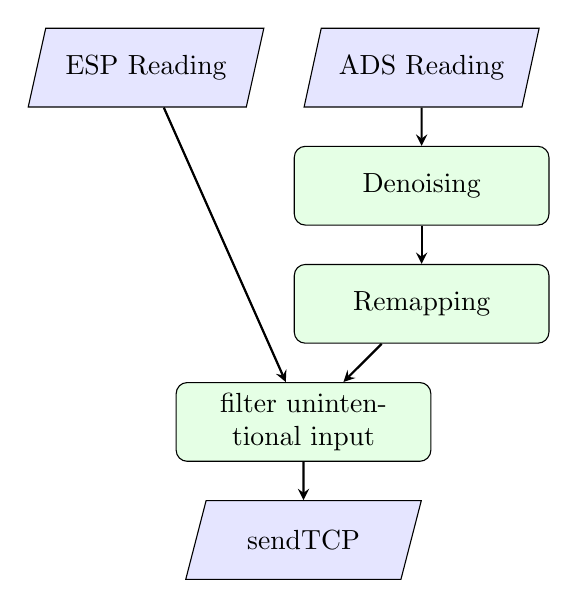
\begin{tikzpicture}[node distance=1.5cm]
	\node (input_esp) [io] {ESP Reading};
	\node (input_ads) [io, right of=input_esp, xshift=2cm] {ADS Reading};
	\node (denoise_ads) [process, below of=input_ads] {Denoising};
	\node (remap_ads) [process, below of=denoise_ads] {Remapping};
	\node (filter_data) [process, below of=input_esp, yshift=-3cm, xshift=2cm] {filter unintentional input};
	\node (send_tcp) [io, below of=filter_data] {sendTCP};

	\draw [arrow] (input_esp) -- (filter_data);
	\draw [arrow] (input_ads) -- (denoise_ads);
	\draw [arrow] (denoise_ads) -- (remap_ads);
	\draw [arrow] (remap_ads) -- (filter_data);
	\draw [arrow] (filter_data) -- (send_tcp);
	\end{tikzpicture}
	\caption{Arduino Datenpipeline}
	\label{fig:arduino_data_pipeline}
\end{minipage}
\end{figure}

In erster Iteration waren auch die Timer für das detektieren multipler Eingaben auf Arduino Seite implementiert, die Behandlung der einzelnen Eingaben auf Unity-Seite wurde auch umgesetzt und getestet.
Die Behandlung der Eingaben erfolgt Statebasiert, für jeden Input gibt es einen Handler, der für jeden von der Uhr gesendeten State also welche App so eben offen ist den korrespondierenden Buttonhandler aufruft.
Beim Testen entschied man sich als Gruppe auch für eine statische Präsentation des Armbandes an einem Schaufensterpuppenarm.\\
Dazu wurde ein 3D Modell eines Armes abgeändert und 3D gedruckt.


\newpage


Beim Testen stellte sich zudem heraus, dass das silberbeschichtete Band, sowie das leitende Garn ohne Probleme in Kombination funktionierten. 
Der piezoresistive Stoff wies bei Positionierung des Silberbandes übereinander das erwartete Verhalten auf, falls jedoch das Band leicht seitlich auf den Sensor drückte, waren die Werte nicht innerhalb des Erwartungsrahmens.
Somit war klar in den nächsten Schritten der Entwicklung musste wert auf die korrekte Positionierung der Sensoren und des Silberbandes geachtet werden.
Der Code für Unity funktionierte auch, womit ich die Sensorik als funktionstüchtig betrachten konnte.
\\
As nächste Iterationen wurde mit der Anzahl der Sensoren variiert, um Sliderbewegungen über weitere Drucksensoren zu realisieren, die dann innerhalb einer Schicht des Armbandes untergebracht werden können. 
Idee war wie im anfänglichen Konzept \ref{fig:concept_layout} weitere Drucksensoren zwischen die bereits existierenden Sensoren zu nähen.
Damit würden Swipebewegung von den Rändern des Armbandes hin zur Mitte beabsichtigt. \\
Es stellte sich nach testweiser Befestigung des Armbandes am Arm heraus, dass die Erkennung der Sequenz der Berührung der Sensoren relativ ungenau war, auch nach verschiedenen Softwaretechnischen Änderungen war dies nicht gut zu beheben, die Auflösung der Sensoren bzw. die Genauigkeit war nicht in der Lage die Swipebewegung in allen Fällen zu erfassen.
Als Konsequenz daraus wurde innerhalb der Gruppe die Idee unterbreitet diese Swipebewegung mit der ''Bezelrotation'' der Smartwatch abzubilden, das wurde dann auch umgesetzt und erwies sich schnell als bessere Interaktion.

\subsection{Konzeptfinalisierung}


\begin{figure}[h]
	\begin{subfigure}[c]{0.33\textwidth}
		\includegraphics[scale=.037]{assets/Strap_fitting_wires.jpg}
		\caption{Sensorplatzierung}
		\label{fig:Initial_drawing1}
	\end{subfigure}
	\begin{subfigure}[c]{0.33\textwidth}
		\includegraphics[scale=.037]{assets/Strap_fitting_sensors.jpg}
		\subcaption{Sensorplatzierung}
		\label{fig:Initial_drawing2}
	\end{subfigure}
		\begin{subfigure}[c]{0.31\textwidth}
		\includegraphics[scale=.037]{assets/Connection_thread_wire.jpg}
		\subcaption{Stromversogung}
		\label{fig:Initial_drawing}
	\end{subfigure}
	\caption{Fitting bracelet to hand3}
\end{figure}
\begin{figure}[h]
	\begin{subfigure}[c]{0.3\textwidth}
		\includegraphics[scale=.037]{assets/Drill_markers.jpg}
		\caption{Verkabelung}
		\label{fig:Initial_drawing4}
	\end{subfigure}
	\begin{subfigure}[c]{0.3\textwidth}
		\includegraphics[scale=.037]{assets/Testing_before_finalizing.jpg}
		\subcaption{Testen der Sensorik}
		\label{fig:Initial_drawing5}
	\end{subfigure}
		\begin{subfigure}[c]{0.3\textwidth}
		\includegraphics[scale=.037]{assets/crop_sensor_fitting.jpg}
		\subcaption{Finaler Prototyp}
		\label{fig:Initial_drawing6}
	\end{subfigure}
	\caption{Fitting bracelet to hand}
\end{figure}

\newpage

Abbildungen \ref{fig:Initial_drawing1} bis \ref{fig:Initial_drawing6} zeigen den Prozess der Finalisierung des Prototyp, dabei wurde zu Beginn die Sensorik platziert und die korrespondierenden Bohrungen vorgenommen, anschließend wurde die unterste Schicht mit der darüberliegenden befestigt und am Arm festgeklebt.
\begin{figure}[ht]
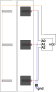
\includegraphics[scale=.3]{assets/final_layout_drawing.jpg}
\caption{ayay}
\label{fig:final_layout}
\end{figure}


\subsection{a}


\newpage

\section{Smartwatch-App Prototyp}

\subsection{Ideenfindung}

Zunächst war für unseren Prototyp keine Smartwatch-App vorgesehen. Auch, da uns dafür die nötige Hardware gefehlt hat und eine Beschaffung nicht in unserem Budget liegen würde. Erst im Gespräch mit unseren Betreuern haben wir eine Samsung Galaxy Gear s3 für die Einbindung in unseren Prototypen in Aussicht gestellt bekommen. Daraufhin mussten wir uns zunächst die Frage stellen, welchen Zweck die Uhr in unserem Produktprototyp erfüllen sollte. Nach einigem Überlegen haben wir uns dazu entschieden, die Smartwatch als zentrales Element unseres Prototyps zu sehen und die auf der Uhr gewählten Anwendungen durch eine Visualisierung und eine Steuerung durch das Armband zu ergänzen. Somit sollte auf der Uhr eine App laufen, die eine Auswahl aus verschiedenen Anwendungen erlaubt. 

\subsection{Lo-Fi-Prototyp}

Als Start in die Umsetzung haben wir zunächst einen Lo-Fi-Prototyp skizziert, um die App, die Sichten und die Navigation zu entwickeln. Dabei ist diese Skizze entstanden (siehe Abbildung \ref{fig:Smatwatch_Prototyp}).

\begin{figure}[h]
	\centering
	\includegraphics[scale=.35]{assets/lo_fo_prototyp.jpeg}
	\caption{Lo-Fi-Prototyp}
	\label{fig:Smatwatch_Prototyp}
\end{figure}

In diesem Lo-Fi-Prototyp waren zunächst drei Sichten definiert. Die Erste sollte ein Home Bildschirm sein. Dies soll ein Default Case sein, in welchem die Smartwatch-App gestartet wird, aber noch keine Anwendung ausgewählt ist. Durch eine Swipe Geste nach rechts oder links, hier durch die Pfeile gekennzeichnet, sollte zwischen den verschiedenen Sichten gewechselt werden können. Die anderen zwei Sichten sollen symbolisieren, dass hier eine Anwendung hinterlegt ist. 

\subsection{Tizen}

Nachdem wir nun also einen ersten theoretischen Prototyp entwickelt hatten, ging es nun an die praktische Implementierung. Dazu mussten wir uns zunächst in die Grundlagen der Tizen Entwicklung einarbeiten und ein neues Projekt aufsetzen. Dabei haben wir uns an dem Watch+Strap Tizen App Projekt der TU Dresden [Quelle: https://github.com/imldresden/WatchStrap-tizen-app] orientiert. 
Nach der Einarbeitung und dem Aufsetzen des neuen Projekts galt es zunächst, die Grundfunktionalitäten der Smartwatch sicherzustellen. Dazu müssten Klassen wie der lowBatterryCheck oder auch die Button-Events für “back” und “main” implementiert werden. 

\subsection{Erstfassung der Smartwatch-App}

Als die Grundfunktionalitäten schließlich implementiert waren, konnten wir uns an die Umsetzung unserer App machen. Dazu haben wir zunächst eine einzelne index.html Seite implementiert, die sich in mehrere sections gegliedert hat. Durch einen Swipe oder durch die Basal Rotation wurde die sectionChange Methode aufgerufen, welche wiederum die nächste section sichtbar gemacht hat. 


\begin{figure}[h]
	\centering
	\includegraphics[scale=.05]{assets/smartwatch_app_erstversion.jpg}
	\caption{Weather Anwendung in früher Version}
	\label{fig:app_erstversion}
\end{figure}

Die Abbildung zeigt beispielhaft eine ausgewählte section, die mit dem Wetter-Icon versehen ist. Das Produkt dieses Abschnittes war eine Tizen-App, die durch Swipegesten oder die Basal Rotation gesteuert durch die sections Home, Weather und Documents bewegt werden konnte. 

\subsection{Websockets}

Als nächster Schritt stand nun die Verbindung zu unserem Unity-Projekt an. Dabei mussten wir zunächst eine geeignete Technologie für unsere Netzwerkübertragung finden. Der erste Versuch war, eine HTTP-Massage zu verschicken. Dies ließ sich zwar aufseiten der Smartwatch-App als Client gut implementieren, dennoch stellte es sich als umständlich heraus, auf Unityseite einen HTTP-Server zu implementieren. Deswegen entschieden wir uns, die Technologie Websockets umzustellen. Nun können folgende Nachrichten von der Smartwatch-App an die Unity-Anwendung verschickt werden: 

\begin{enumerate}
	\item{“0” - Home section / zurück auf Home section}	
	\item{“1” - weather section}
	\item{“2” - graph section}
	\item{“3” - documents section}
	\item{“a1” - weather Anwendung gestartet}
	\item{“a2” - graph Anwendung gestartet}
	\item{“a3” - documents Anwendung gestartet}
	\item{“cw” - Clockwise Rotation}
	\item{“ccw” - counterClockwise Rotation}
\end{enumerate}

Auf Seiten von Unity gibt es einen mit WebSocketSharp erstellten Websocket-Server. Dieser kann die Nachrichten empfangen und in der Methode StateChange.SetAppState() zur Weiterverarbeitung in Unity zur Verfügung stellen. 

\subsection{Zweitfassung der Smartwatch-App}

Nachdem die Websocket-Kommunikation implementiert war, kam noch der Wunsch auf, auch innerhalb der einzelnen Anwendungen die Basal-Rotation zur Steuerung der Visualisierung nutzen zu können. Deswegen braucht es eine Trennung zwischen der Anwendungsauswahl, die ebenfalls über die Basal-Rotation möglich ist, und der Anwendung selbst. Aus diesem Grund haben wir einen Button auf das jeweilige App-Auswahlfeld gemacht, der eine HTML-Unterseite aufruft, die eigene Scripte lädt und so eine Trennung von der Auswahl einer App und dem "in einer App sein" ermöglicht. 

\begin{figure}[h]
	\centering
	\includegraphics[scale=.05]{assets/smartwatch_app_zweitversion.jpg}
	\caption{Finale Documents Anwendung}
	\label{fig:app_zweitversion}
\end{figure}

Wie in der Abbildung zu erkennen, haben wir die Anwendungsseite auch farblich an die Visualisierung angelehnt gestaltet, um so auch visuell noch eine Verbindung zwischen der Smartwatch-App und der Unitiy Visualisierung zu schaffen. 

\subsection{Systemintegration}

Die Smartwatch-App gliedert sich in das Gesamtprojekt als Element zur Anwendungsauswahl und zur Steuerung ein. So kann über die App eine Unter-Anwendung Weather, Graph oder Documents ausgewählt und durch einen Button-Klick gestartet werden. Durch die Basal-Rotation können bestimmte Elemente der Visualisierung darüber hinaus auch gesteuert werden. Außerdem kann über den Home Button eine Anwendung wieder geschlossen werden. 


\newpage

\listoffigures
% list tables if used
%\listoftables

\end{document}